% Project 2 - EECS 499
% Author: Shaun Howard (smh150@case.edu)
\documentclass[conference]{IEEEtran} \usepackage[T1]{fontenc} \usepackage[backend=biber, style=ieee]{biblatex}
\addbibresource{report.bib} \usepackage[final]{microtype}

% graphics
\ifCLASSINFOpdf \usepackage[pdftex]{graphicx} % declare the path(s) where your graphic files are
  \graphicspath{{images/}} % and their extensions so you won't have to specify these with
  % every instance of \includegraphics
  \DeclareGraphicsExtensions{.jpeg,.png} \else
\fi


\begin{document}

\title{Online Jacobian and Randomized-IK RRT Path Planning for Baxter Dual Arm Manipulation}

\author{
 \IEEEauthorblockN{Shaun Howard}
 \IEEEauthorblockA{Electrical Engineering and Computer Science Department\\
                   Case Western Reserve University\\ 
                   Cleveland, Ohio 44106\\
                   Email: smh150@case.edu}
}

% make the title area
\maketitle

% As a general rule, do not put math, special symbols or citations
% in the abstract
\begin{abstract}
Within this paper a more flexible solution to the path planning problem for multi-arm robots is presented. Modifications were made to the concept of a Rapidly-
exploring Random Tree necessary to fuse several successful Jacobian-based techniques for redundant manipulator planning. This hybrid RRT planner uses the fusion 
of Jacobian-Transpose and Jacobian-Pseudoinverse-based methods for goal-directed path planning. For random path planning, a IK straight-line solver is used to 
sample solutions at random points within growing radii from the goal center until a goal is found or the maximum number of retires is met. The pairing of the 
hybrid RRT and random IK-based planner methods allow solutions to be found very quickly if possible, otherwise, the planner will get as close as possible over 
time or a minimum distance threshold is met. This method was found to perform better than the Jacobian-Transpose and IK-based approaches overall, although each 
method has upsides and downsides. Rarely, if ever, does the planner get noticeably stuck in local minima unless a goal is impossible for the end effector to 
reach. A Gazebo simulation paired with Rviz is used to examine custom implementations of the algorithms mentioned. A comparison is made between the methods used 
during experimentation which reveals that the hybrid RRT planner is quicker than the other planning methods while balancing constraints and generating a viable solution to almost any problem within reach of the given end effector in use.
\end{abstract}

\section{Introduction} \label{Introduction}

The concept of real-time path planning in robotics has stirred a lot of research in recent years. <author> 

\begin{figure}
\label{pic1} 
\centering 
% 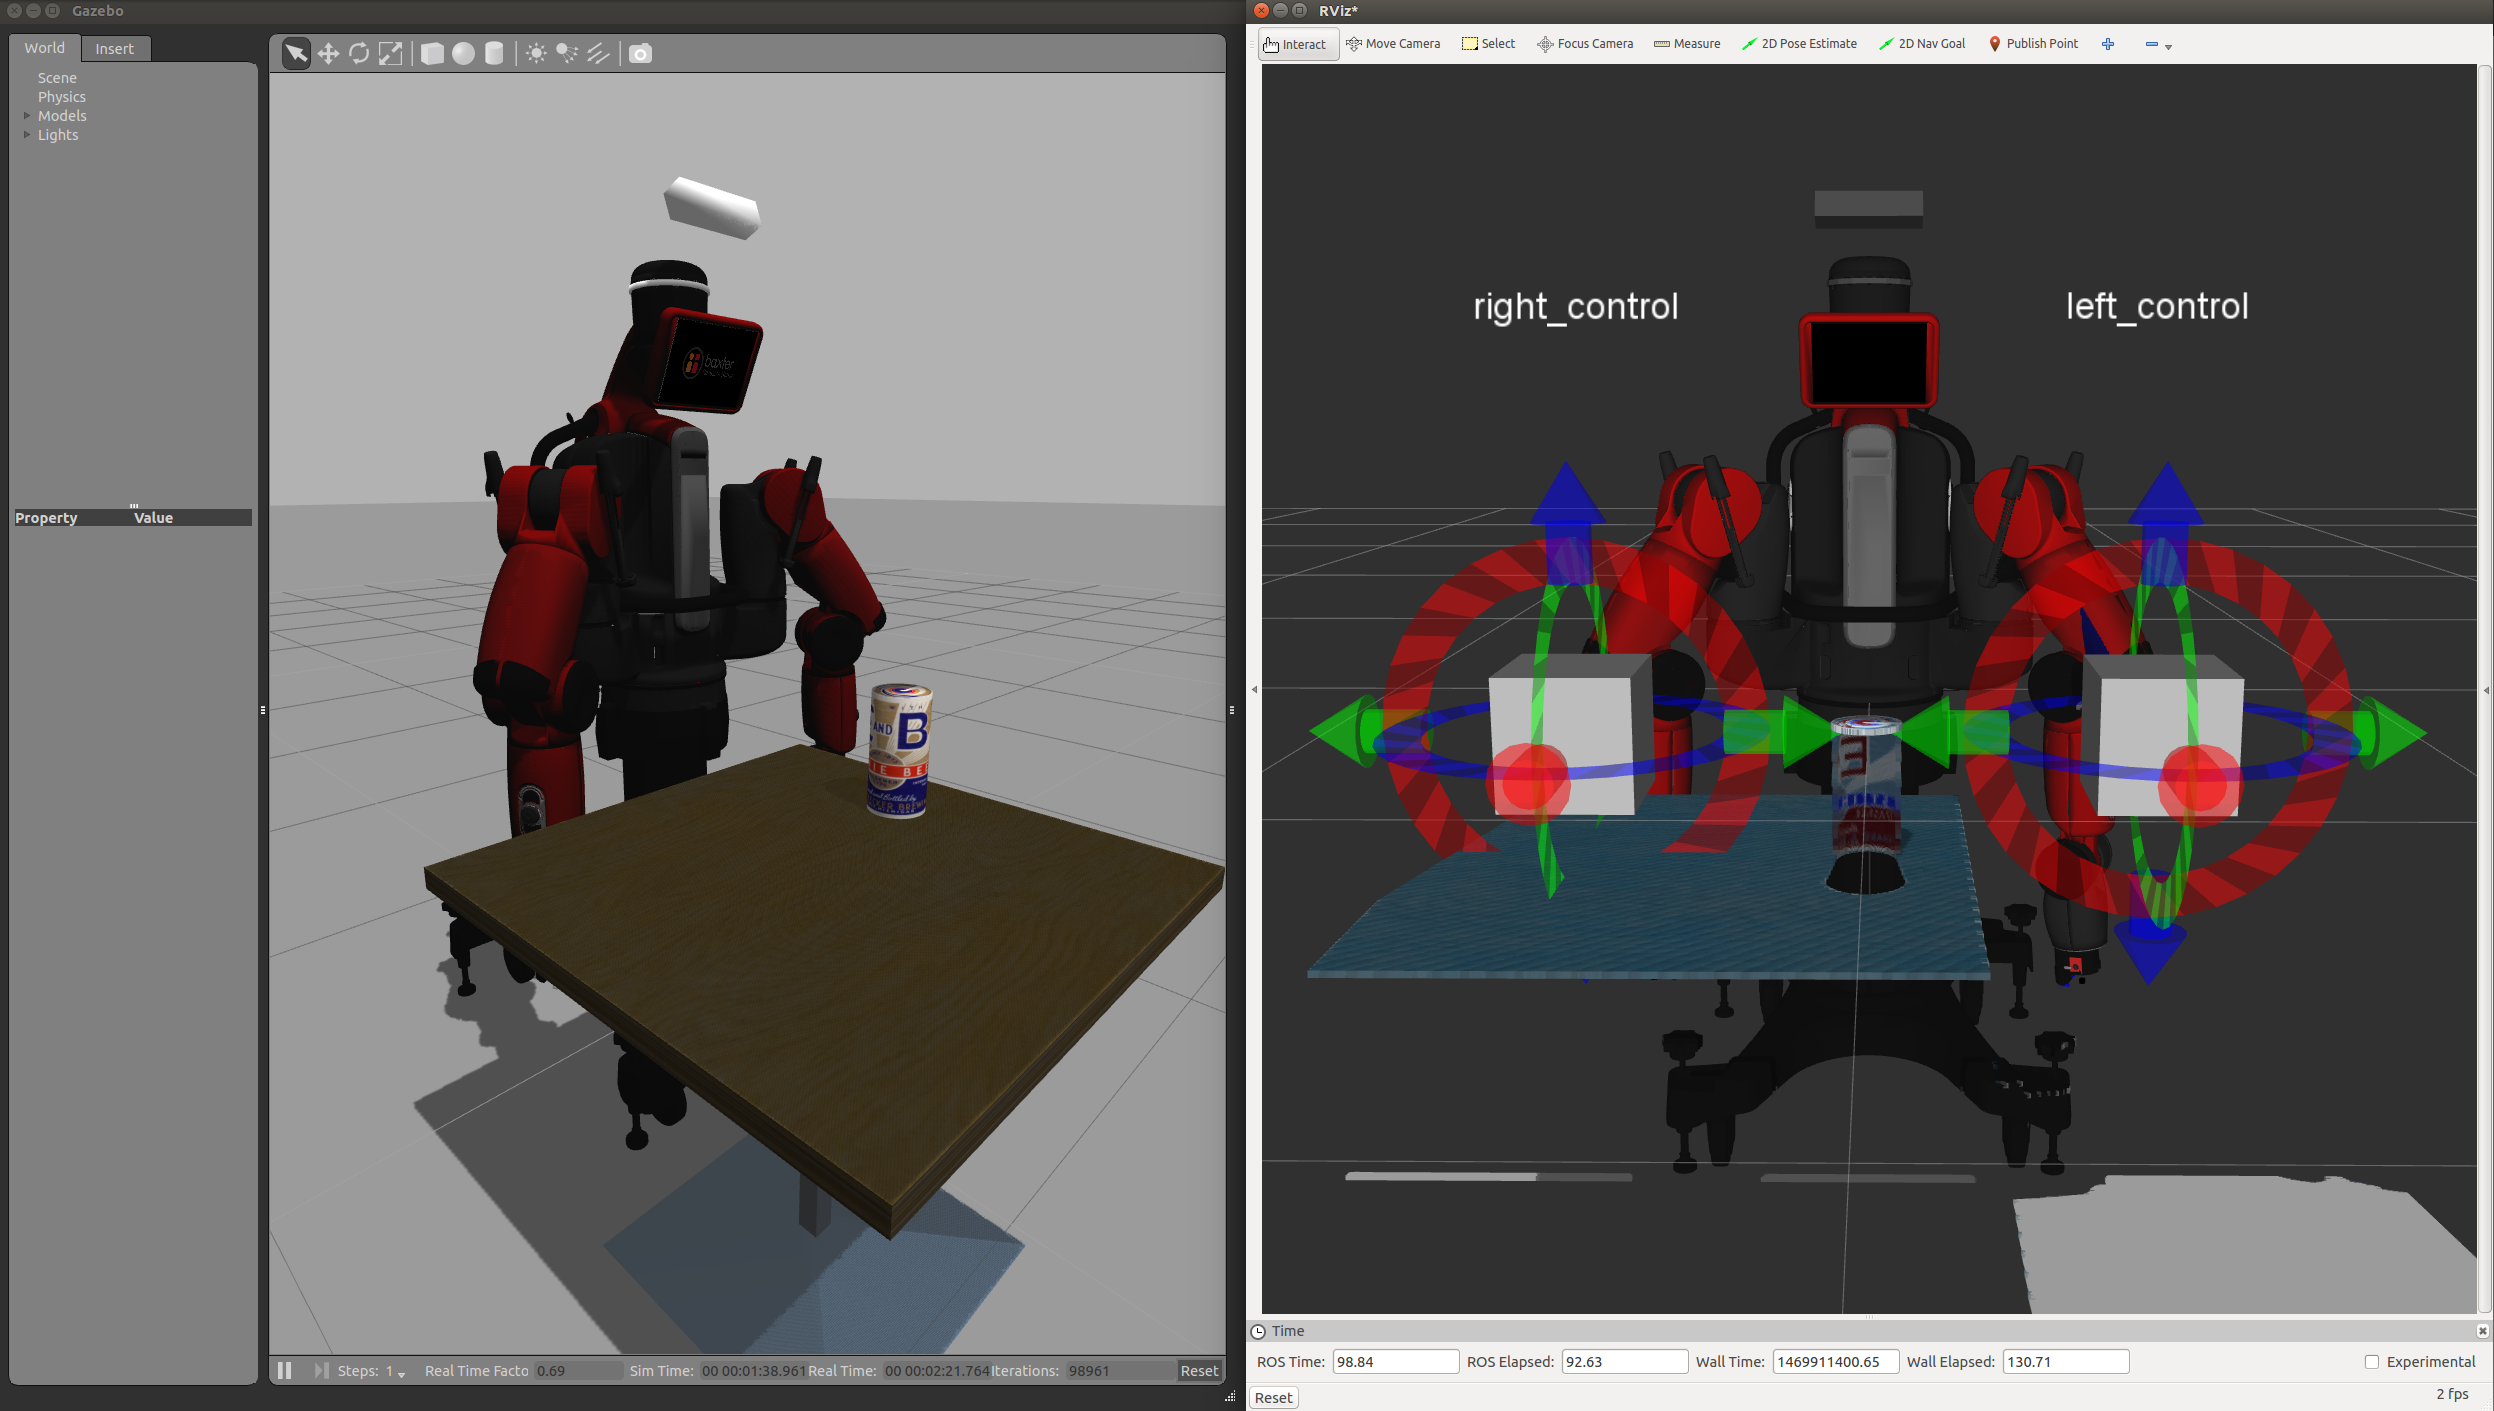
\includegraphics[width=0.49\textwidth]{sim1}
\caption{A squadron S of three TurtleBot 2's on a grid-based world attempt to estimate the position of R, the middle moving TurtleBot 2.}
\end{figure}

\section{Related Work} \label{Related Work}

\section{Problem Formulation} \label{Problem Formulation}

\section{Methodology} \label{Methodology}

\subsection{Sensor Measurements} \label{Sensor Measurements}

\subsection{Planner Implementation} \label{Planner Implementation}

\subsection{Gazebo Simulation} \label{Gazebo Simulation}

\section{Conclusion} \label{Conclusion} 

\subsection{Future Work}

\printbibliography
\end{document}